\chapter{An attempt at Reinforcement Learning of Policies}
\section{Grid World tabular solutions}
In this section, for the sake of example, we assume that a dictionary with 4 key-value pais is less interpretable than a depth-1 decision tree.
In Figure~\ref{fig:optimal-policy}, we illustrate \textit{a}--there are others--tabular optimal policy for the grid world MDP described in the previous section, i.e. that maximizes the objective (cite). 
In any starting state, the agent will move towards the abosrbing state with positive reward.
\begin{figure}[ht]
\centering
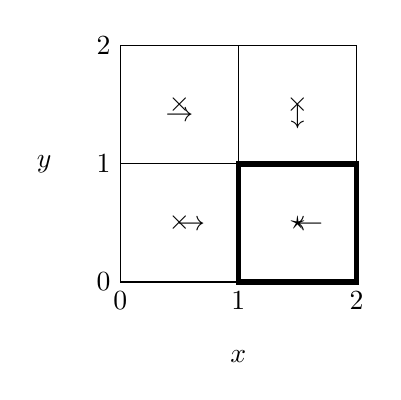
\begin{tikzpicture}[scale=1.5]
    % Draw the grid cells
    \draw (0,0) grid (2,2);
    
    % Add ticks on axes
    \foreach \x in {0,1,2}
        \node[below] at (\x,0) {$\x$};
    \foreach \y in {0,1,2}
        \node[left] at (0,\y) {$\y$};
    
    \node[left] at (-0.5, 1) {$y$};
    \node[below] at (1, -0.5) {$x$};
    
    % Label cells
    \node at (0.5,0.5) {$\times$};
    \node at (0.6,0.48) {$\rightarrow$};

    \node at (0.5,1.5) {$\times$};
    \node at (0.5,1.4) {$\rightarrow$};

    \node at (1.5,1.5) {$\times$};
    \node at (1.5,1.4) {$\downarrow$};
    
    % Goal state in bottom right with double border
    \draw[line width=2pt] (1,0) rectangle (2,1);
    \node at (1.5,0.5) {$\star$};
    \node at (1.6,0.48) {$\leftarrow$};

    
\end{tikzpicture}
\caption{An optimal tabular policy for the grid world.}\label{fig:optimal-policy}
\end{figure}


\begin{figure}[htbp]
    \centering
    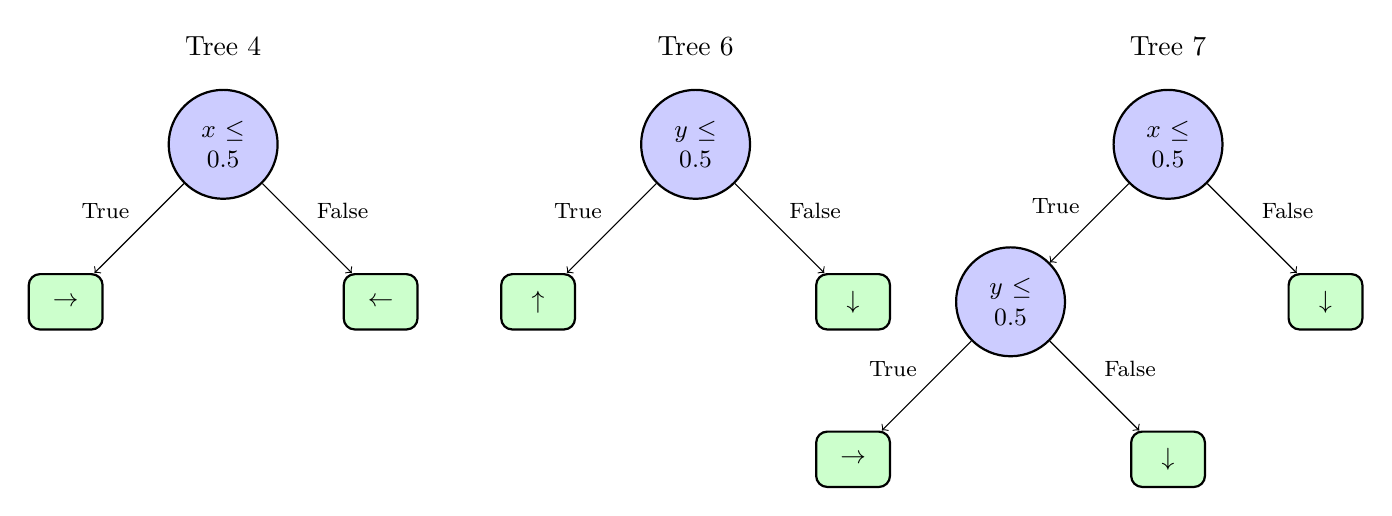
\begin{tikzpicture}[
        scale=1.0,
        decision/.style={circle, draw, thick, fill=blue!20, text width=2.5em, text centered, minimum height=2.5em, font=\small},
        leaf/.style={rectangle, draw, thick, fill=green!20, text width=2em, text centered, rounded corners, minimum height=2em, font=\small},
        edge_label/.style={font=\footnotesize, midway}
    ]
        % Tree 4: if x <= 0.5 move right else move left
        \node[decision] (tree4_root) at (0,0) {$x \leq 0.5$};
        \node[leaf] (tree4_right) at (-2,-2) {$\rightarrow$};
        \node[leaf] (tree4_left) at (2,-2) {$\leftarrow$};
        \draw[->] (tree4_root) -- (tree4_right) node[edge_label, above left] {True};
        \draw[->] (tree4_root) -- (tree4_left) node[edge_label, above right] {False};

        % Tree 6: if y <= 0.5 move up else move down
        \node[decision] (tree6_root) at (6,0) {$y \leq 0.5$};
        \node[leaf] (tree6_up) at (4,-2) {$\uparrow$};
        \node[leaf] (tree6_down) at (8,-2) {$\downarrow$};
        \draw[->] (tree6_root) -- (tree6_up) node[edge_label, above left] {True};
        \draw[->] (tree6_root) -- (tree6_down) node[edge_label, above right] {False};

        % Tree 7: if x <= 0.5 and y <= 0.5 move right else move down
        \node[decision] (tree7_root) at (12,0) {$x \leq 0.5$};
        \node[decision] (tree7_y) at (10,-2) {$y \leq 0.5$};
        \node[leaf] (tree7_right) at (8,-4) {$\rightarrow$};
        \node[leaf] (tree7_down) at (12,-4) {$\downarrow$};
        \node[leaf] (tree7_down2) at (14,-2) {$\downarrow$};
        \draw[->] (tree7_root) -- (tree7_y) node[edge_label, above left] {True};
        \draw[->] (tree7_root) -- (tree7_down2) node[edge_label, above right] {False};
        \draw[->] (tree7_y) -- (tree7_right) node[edge_label, above left] {True};
        \draw[->] (tree7_y) -- (tree7_down) node[edge_label, above right] {False};

        % Labels
        \node[above] at (0,1) {Tree 4};
        \node[above] at (6,1) {Tree 6};
        \node[above] at (12,1) {Tree 7};
    \end{tikzpicture}
    \caption{Some optimal decision tree policies.}
    \label{fig:optimal-policy-trees}
\end{figure}

For this grid world, there exist \textit{optimal} decision tree policies. 
In particular Tree 4 and 6 are have very good interpretability-performance trade-offs (smallest tree that can get the maximum MDP reward).
In the rest of this section we shall attempt to \textit{learn} those trees from data. 


\begin{figure}[htbp]
    \centering
    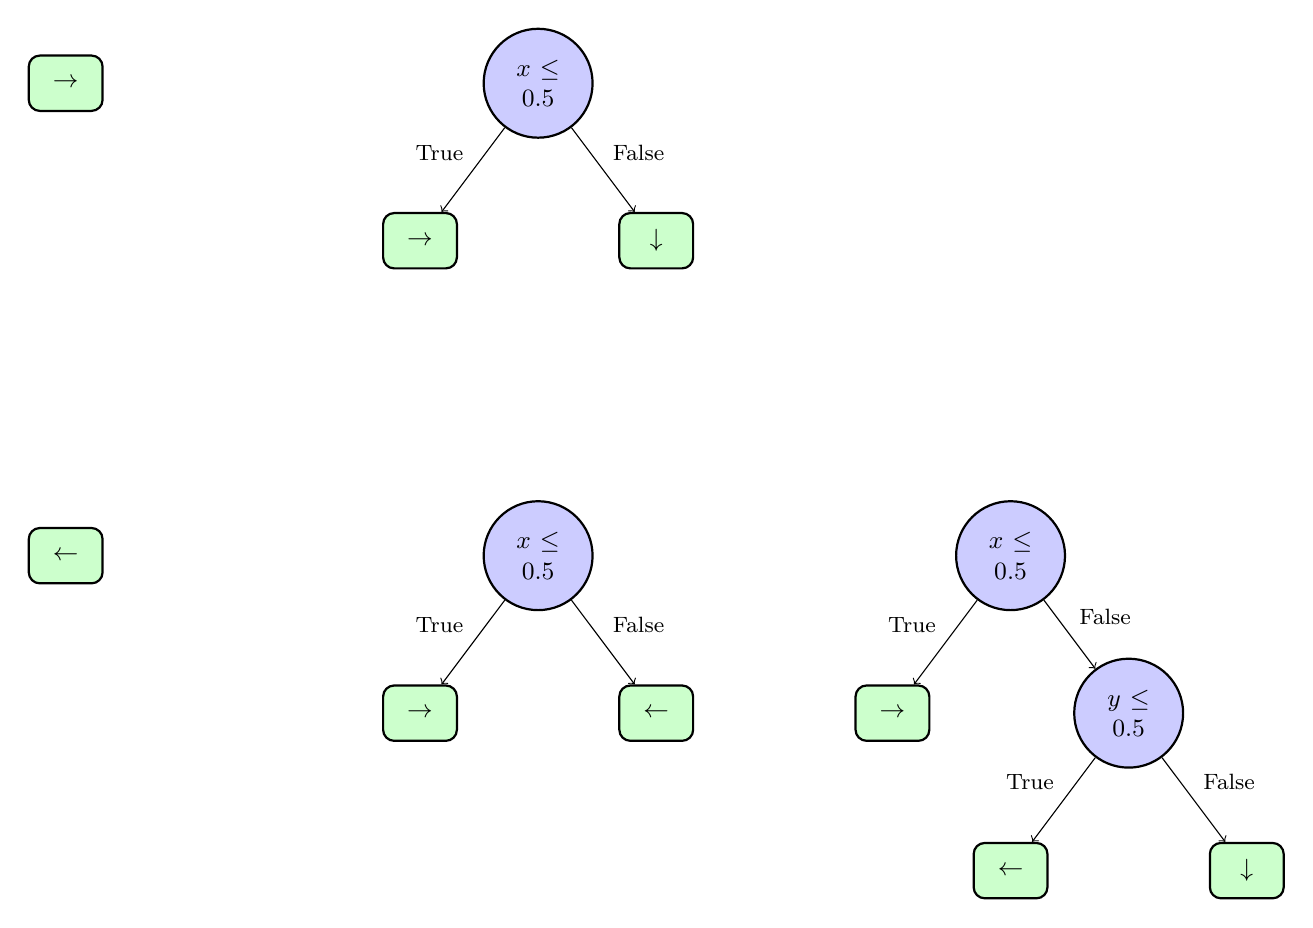
\begin{tikzpicture}[
        scale=1.0,
        decision/.style={circle, draw, thick, fill=blue!20, text width=2.5em, text centered, minimum height=2.5em, font=\small},
        leaf/.style={rectangle, draw, thick, fill=green!20, text width=2em, text centered, rounded corners, minimum height=2em, font=\small},
        edge_label/.style={font=\footnotesize, midway}
    ]
        % Tree 1: Move Right
        \node[leaf] (tree1) at (0,0) {$\rightarrow$};

        % Tree 3: if x <= 0.5 move right else move down
        \node[decision] (tree3_root) at (6,0) {$x \leq 0.5$};
        \node[leaf] (tree3_right) at (4.5,-2) {$\rightarrow$};
        \node[leaf] (tree3_down) at (7.5,-2) {$\downarrow$};
        \draw[->] (tree3_root) -- (tree3_right) node[edge_label, above left] {True};
        \draw[->] (tree3_root) -- (tree3_down) node[edge_label, above right] {False};

        % Tree 2: Move Left
        \node[leaf] (tree2) at (0,-6) {$\leftarrow$};

        % Tree 4: if x <= 0.5 move right else move left
        \node[decision] (tree4_root) at (6,-6) {$x \leq 0.5$};
        \node[leaf] (tree4_right) at (4.5,-8) {$\rightarrow$};
        \node[leaf] (tree4_left) at (7.5,-8) {$\leftarrow$};
        \draw[->] (tree4_root) -- (tree4_right) node[edge_label, above left] {True};
        \draw[->] (tree4_root) -- (tree4_left) node[edge_label, above right] {False};

        % Tree 5: if x <= 0.5: move right elif y <= 0.5 move left else move down
        \node[decision] (tree5_root) at (12,-6) {$x \leq 0.5$};
        \node[leaf] (tree5_right) at (10.5,-8) {$\rightarrow$};
        \node[decision] (tree5_y) at (13.5,-8) {$y \leq 0.5$};
        \node[leaf] (tree5_left) at (12,-10) {$\leftarrow$};
        \node[leaf] (tree5_down) at (15,-10) {$\downarrow$};
        \draw[->] (tree5_root) -- (tree5_right) node[edge_label, above left] {True};
        \draw[->] (tree5_root) -- (tree5_y) node[edge_label, above right] {False};
        \draw[->] (tree5_y) -- (tree5_left) node[edge_label, above left] {True};
        \draw[->] (tree5_y) -- (tree5_down) node[edge_label, above right] {False};
    \end{tikzpicture}
    \caption{Examples of decision trees for different policies in the grid world. Each tree represents a different policy, from simple single-action policies to more complex conditional policies.}
    \label{fig:policy-trees}
\end{figure}


\section{Method}
Let us compute the objective value (cite) for the trees presented above. We will identify the range of $\zeta$ values--the interpretabiliy penalty--for which the depth-1 tree is optimal. 
Let us compute the objective values of the most rewarded tree for each tree structure.
\paragraph{Depth-0 decision tree:} has only one leaf node that takes a single base action indefinitely.
For this type of tree the best reward achievable is to take actions that maximize the probability of reaching the objective $\rightarrow$ or $\downarrow$. In that case the objective value of such tree is:
In the goal state $(1, 0)$, the value of the depth-0 tree $\mathcal{T}_0$ is:
\begin{align*}
    V^{\mathcal{T}_0}_g &= 1 + \gamma + \gamma ** 2 \\
    &= \frac{1}{1 - gamma}
\end{align*}
In the state $(0, 0)$ when the policy repeats going right respectively in the state $(0, 1)$ when the policy reoeats going down, the value is:
\begin{align*}
    V^{\mathcal{T}_0}_{(0, 0)} &= 0 + \gamma V^{\mathcal{T}_0}_g
    &= \gamma V^{\mathcal{T}_0}_g
\end{align*}
In the other states the policy never gets positive rewards. Hence:
\begin{align*}
J(\mathcal{T}_0) &= \frac{1}{4} V^{\mathcal{T}_0}_g + \frac{1}{4} V^{\mathcal{T}_0}_{(0, 0)}
\end{align*}
\section{Results}

We first start by plotting the learning curves of three classical RL algorithms described in the preliminaries. There was a series of work in the 1990's(cite) that studied the performances of RL algos when naively applied to he partially observable setting, i.e, naively setting $s\leftarrow o$.
The key observations are:
\begin{enumerate}
    \item The learning finishes, i.e, learning curves flatten after some iterations.
    \item There is a shift between the policies learned between the depth-0 tree and the depth>1 trees when $\zeta\geq0$.
\end{enumerate}
This is problematic because we know that \textit{theoretically}, for $0<\zeta<1$, the optimal policy for the IBMDP objective had depth $= 1$.
